\documentclass[letterpaper]{article}

\usepackage[utf8]{inputenc}
\usepackage[sort, colon]{natbib}
\usepackage{alifexi}
\usepackage[bottom]{footmisc}
\usepackage[colorlinks=true,citecolor=green,linkcolor=blue]{hyperref}
\usepackage[font=scriptsize,labelfont=bf]{caption}
\usepackage{tabulary}
\usepackage{flushend}

\usepackage{mathtools}
\usepackage{commath}

\usepackage{dblfloatfix}

\title{Reproducing and updating results from
\textit{Uncovering disease-disease relationships\\through the incomplete interactome}}
\author{Robin Petit$^{1}$ \and Tom Lenaerts$^{1}$\\
\mbox{}\\
$^1$Université Libre de Bruxelles}


\begin{document}
\maketitle

\begin{abstract}
This paper intends to reproduce some of the results of the article \textit{Uncovering
disease-disease relationships through the incomplete interactome} \citep{originalPaper}
and check the robustness of the procedure by comparing the results obtained with the data
of the original paper with the results obtained with updated datasets. As the analysis of
the original paper intends to be systematic, it is important to observe the effect of a
more recent version of the interactome on the results and their significance. We found that
the results of the paper, while being reproducible, are affected by the use of a more recent
interactome, mainly on the number of significant results.
\end{abstract}

\section{Introduction}
An interactome is a graph containing all the biologically relevant molecular interactions found within
a cell. This notion first appeared in 1999 for the drosophila \citep{sanchez1999grasping} and the need
to thoroughly study this structure has been expressed less than 15 years ago
\citep{UnderstandingTheCellFunctionalOrganization}.

The interactome is one of many biological networks. Among others, we can find the genome, covering
gene networks \citep{boucher2013genetic}, the proteome for the protein networks
\citep{rolland2014proteome}, disease networks \citep{goh2007human}. Biological networks provide the
ability to deeply study biology \citep{UnderstandingTheCellFunctionalOrganization}, as well as
medicine \citep{barabasi2011network} and, more recently, pharmacology \citep{hopkins2008network}.

Diseases are considered as the result of an interplay between molecular interactions. The need to use
the interactome as a tool to analyze genetic diseases behaviour had already been expressed several years
ago \citep{vidal2011interactome}. However, the interactome is incomplete and estimated around $20\%$-complete
for the interactions involved and around $54\%$-complete for the proteins involved
\citep{ATruerMeasureOfOurIgnorance,estimatingTheSizeOfTheHumanInteractome}. The authors of the original paper
\citep{originalPaper} showed that the human interactome has now reached sufficient completion to systematically
study diseases. Moreover, the interactome now allows the study of many more genetic relations, such as
drug-disease correlation \citep{Yu2016extraction} or digenic diseases \citep{gazzo2015dida}.

In the original paper, authors extracted genes associated with diseases from several disease genes
association databases, in particular OMIM, the Online Mandelian Inheritance in Man \citep{amberger2008OMIM},
and GWAS, the Genome-Wide Association Studies, compiled by PhenGenI \citep{ramos2014PhenGenI}. These
genes were mapped on the human interactome in order to determine the properties of these disease modules
in the graph. They discovered firstly that diseases tend to \textit{cluster} in denser subgraphs than
the interactome itself and secondly that phenotypically close diseases tend to overlap on a significant
amount of genes.

The first part of this paper focuses on the reproduction of some of the results of the original paper,
namely the disease modules propensity to cluster into highly connected components and the significantly
lower separation indicator values for highly gene related disease pairs. The second part will reproduce
the results with an updated interactome in order to test the robustness of the analysis. In the third
part, we will discuss an analytical way of determining simulations results.

\section{Results}
	\subsection{Reproducibility}\label{subsec:reproducibility}
	The interactome used in the original paper contains 13,460 genes and 141,296 physical interactions
	constructed on several interactions databases including BioGRID \citep{chatr2017biogrid}, IntAct
	\citep{kerrien2011intact}, TRANSFAC \citep{matys2003transfac}, MINT \citep{licata2011mint}, HPRD
	\citep{keshava2008HPRD}, KEGG and BIGG \citep{lee2008KEGG-BIGG}, CORUM \citep{ruepp2009corum} and
	PhosphitePlus \citep{hornbeck2011phosphositeplus}.

	Authors chose to rely only on physical protein-protein interactions (PPI) and to exclude functional
	interactions \citep{caldera2017interactome}. This interactome is available for download in the
	supplementary material.

	The diseases studied are selected such that they possess at least 20 genes associated to them.
	We obtained 29,775 disease-gene associations on 3,173 distinct genes, with 2,436 genes found in the
	interactome.

		\subsubsection{Clustering of disease modules}
		The original paper discusses the tendency of the diseases to cluster into dense subgraphs. In order
		to check this hypothesis, we analyzed the largest connected component (LCC) of the diseases in the
		interactome. We compared the relative size of the module, defined by $r = S/N_d$, with $S$ the size
		of the LCC of the disease, and $N_d$, the number of genes associated with the given disease, with
		the $z$-score of the LCC size of a disease, which is computed by comparing the relative size of the
		module with the size of the largest LCC of the disease obtained by chance (Figure~\ref{fig:zscore}).

		We observed that 241 out of the 299 diseases (more than $80\%$) have a significantly bigger LCC than
		expected by chance. The $z$-score of the LCC size of a disease is strongly related to its relative
		module size.

		\begin{figure}[!h]
			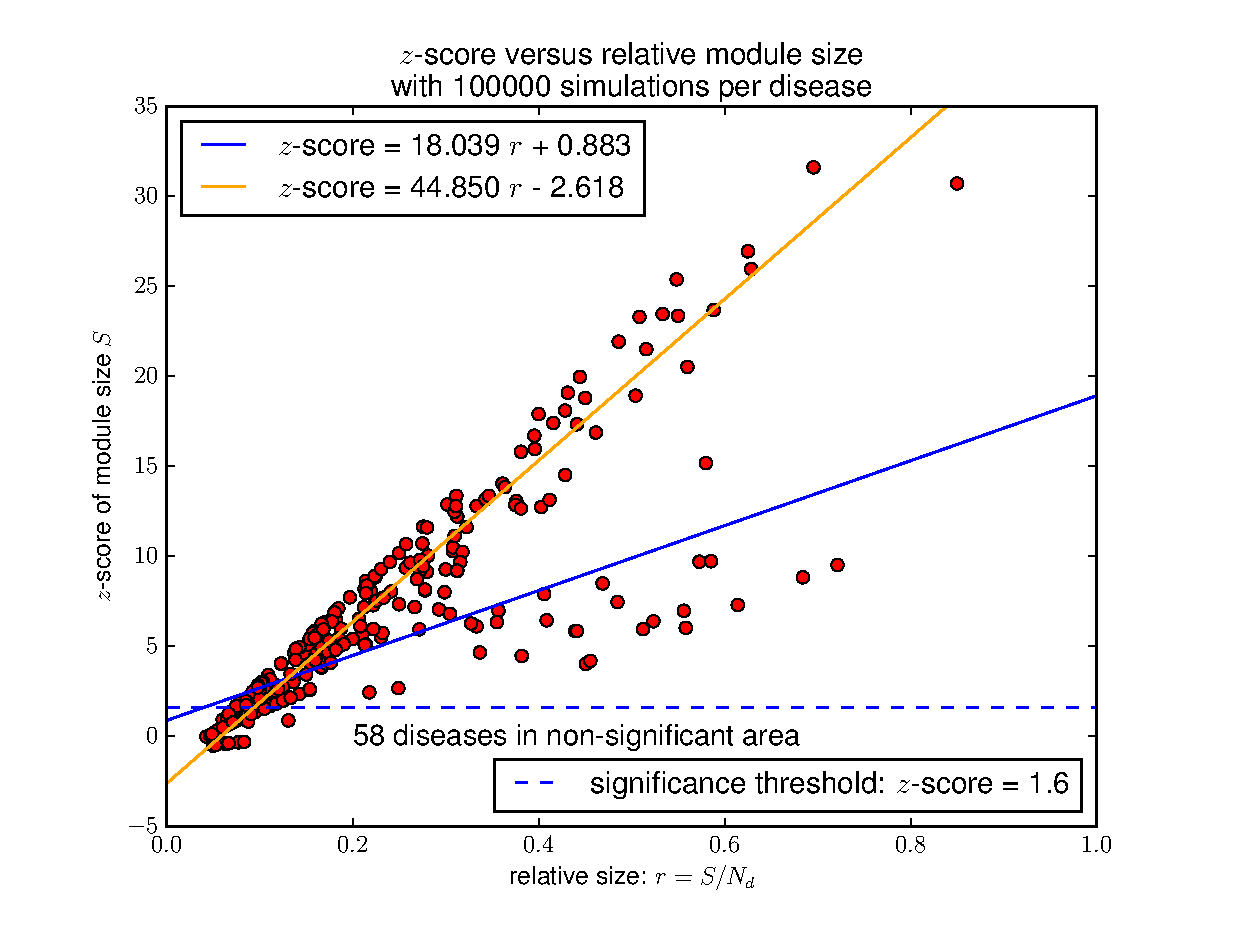
\includegraphics[width=.5\textwidth]{images/S4.b100000.eps}
			\vspace{-.7cm}
			\caption{\textbf {$z$-score of largest connected component size vs relative module size.}
			100,000 simulations have been performed per disease in order to determine the size of the largest
			connected component of the disease subgraph expected by chance. Diseases being highly connected,
			thus highly covered by the interactome, present a higher $z$-score and then a higher confidence
			about the significance of the clustering observed. Assuming that the distribution of largest
			connected component is normal for random samples \citep{fluctuationGiantComponent}, each $z$-score
			can be associated to a $p$-value, in particular, $z$-score $\geq 1.6$ corresponds to $p$-value
			$\leq 0.05$, representing significance threshold (dotted line in the plot).
			\label{fig:zscore}}
		\end{figure}

		We observed that several diseases do not present a significantly larger largest connected component
		than expected by chance. These diseases have a small relative size, less than $20\%$ of their related
		genes are connected in the current interactome. On the other hand, diseases with bigger relative size
		have a higher $z$-score, leading us to think that a more complete interactome, with higher coverage
		of the diseases could increase the significance of the result.

		These results confirm the observation of the original paper that disease modules tend to cluster.

		\subsubsection{Separation distribution}
		The original paper describes the separation of diseases in the interactome through two different
		measures. The first one is the overlapping scores, $C$-score and $J$-score, defined respectively as
		$\abs {A \cap B}/\min(\abs A, \abs B)$ and $\abs {A \cap B}/\abs {A \cup B}$ for $A$ and $B$ two
		disease genes sets. The second one is the separation score, $s_{AB}$, defined as follows :
		\begin{equation}
			s_{AB} = \langle d_{AB} \rangle - \frac {\langle d_A \rangle + \langle d_B \rangle}{2}.
		\end{equation}
		for two diseases $A$ and $B$, with $\langle d_A \rangle$ and $\langle d_B \rangle$ as the mean
		distance between two proteins in the disease subgraphs of $A$ and $B$ respectively, and with
		$\langle d_{AB} \rangle$ as the mean distance between two proteins of each disease subgraph.

		\begin{table}
		\begin{tabular}{m{.1\textwidth}|m{.1\textwidth}|m{.08\textwidth}|m{.08\textwidth}}
			$J = 0$ & $0 < J < 1$ & $J < 1$ & $J = 1$ \\
			$C = 0$ & $0 < C < 1$ & $C = 1$ & $C = 1$ \\
			\hline
			\hline
			No common gene & Partial overlap & $A$ is complete subset of $B$ & $A$ and $B$ are identical
		\end{tabular}
		\caption{Meaning of the different $J$-score/$C$-score combinations.\label{tab:J-C-scores}}
		\end{table}

		\begin{figure}[!h]
		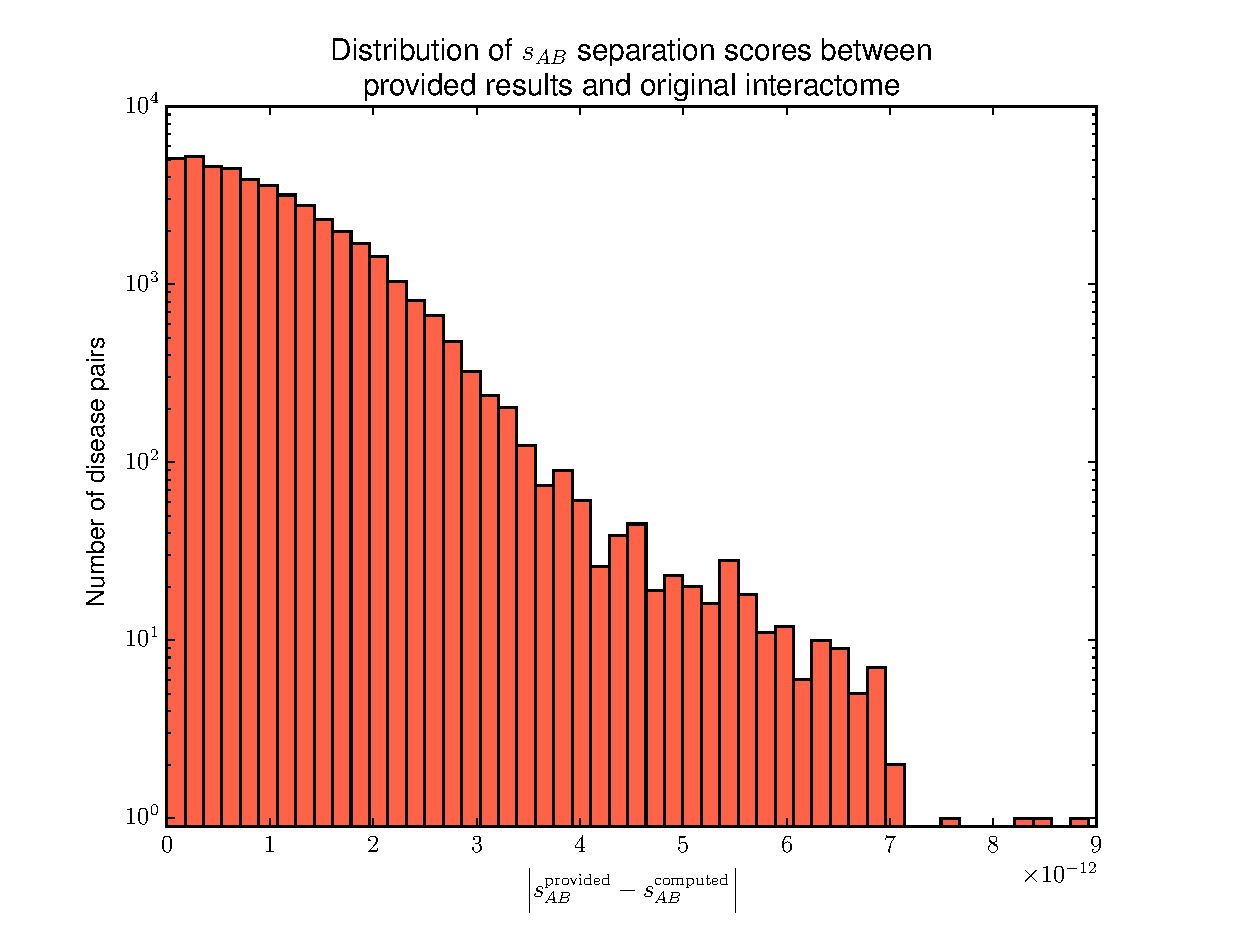
\includegraphics[width=.5\textwidth]{images/sep_difference_histogram.eps}
		\vspace{-.5cm}
		\caption{{\bf Distribution of the difference between the provided $s_{AB}$ score and the computed
		$s_{AB}$ score.} We observe that difference is very small, below $10^{-11}$, which can be ascribed
		to computation precision.
		\label{fig:s_AB difference}}
		\end{figure}

		We analyzed the distribution of the number of disease pairs separated into different groups according
		to the combination of their overlapping scores (Table~\ref{tab:J-C-scores}) according to their
		separation score (Figure~\ref{fig:s_AB histogram}). We found similar results to the ones in the
		original paper, with the fact that diseases sharing no common genes are also mainly separated
		($s_{AB} > 0$), even though some modules overlap. However, complete overlap of the modules showed a
		great diversity of separating scores. The only difference observed was that for non-overlapping
		disease pairs, the amount of pairs having a separation value below 0 is $710$ versus $717$ in the
		original paper, which is due to computation precision since all computed separation values deviate
		by less than $10^{-11}$ from provided values by authors of the original paper
		(Figure~\ref{fig:s_AB difference}).

		\begin{figure*}[!t]
			\hspace{-1.8cm}
			\vspace{-1cm}
			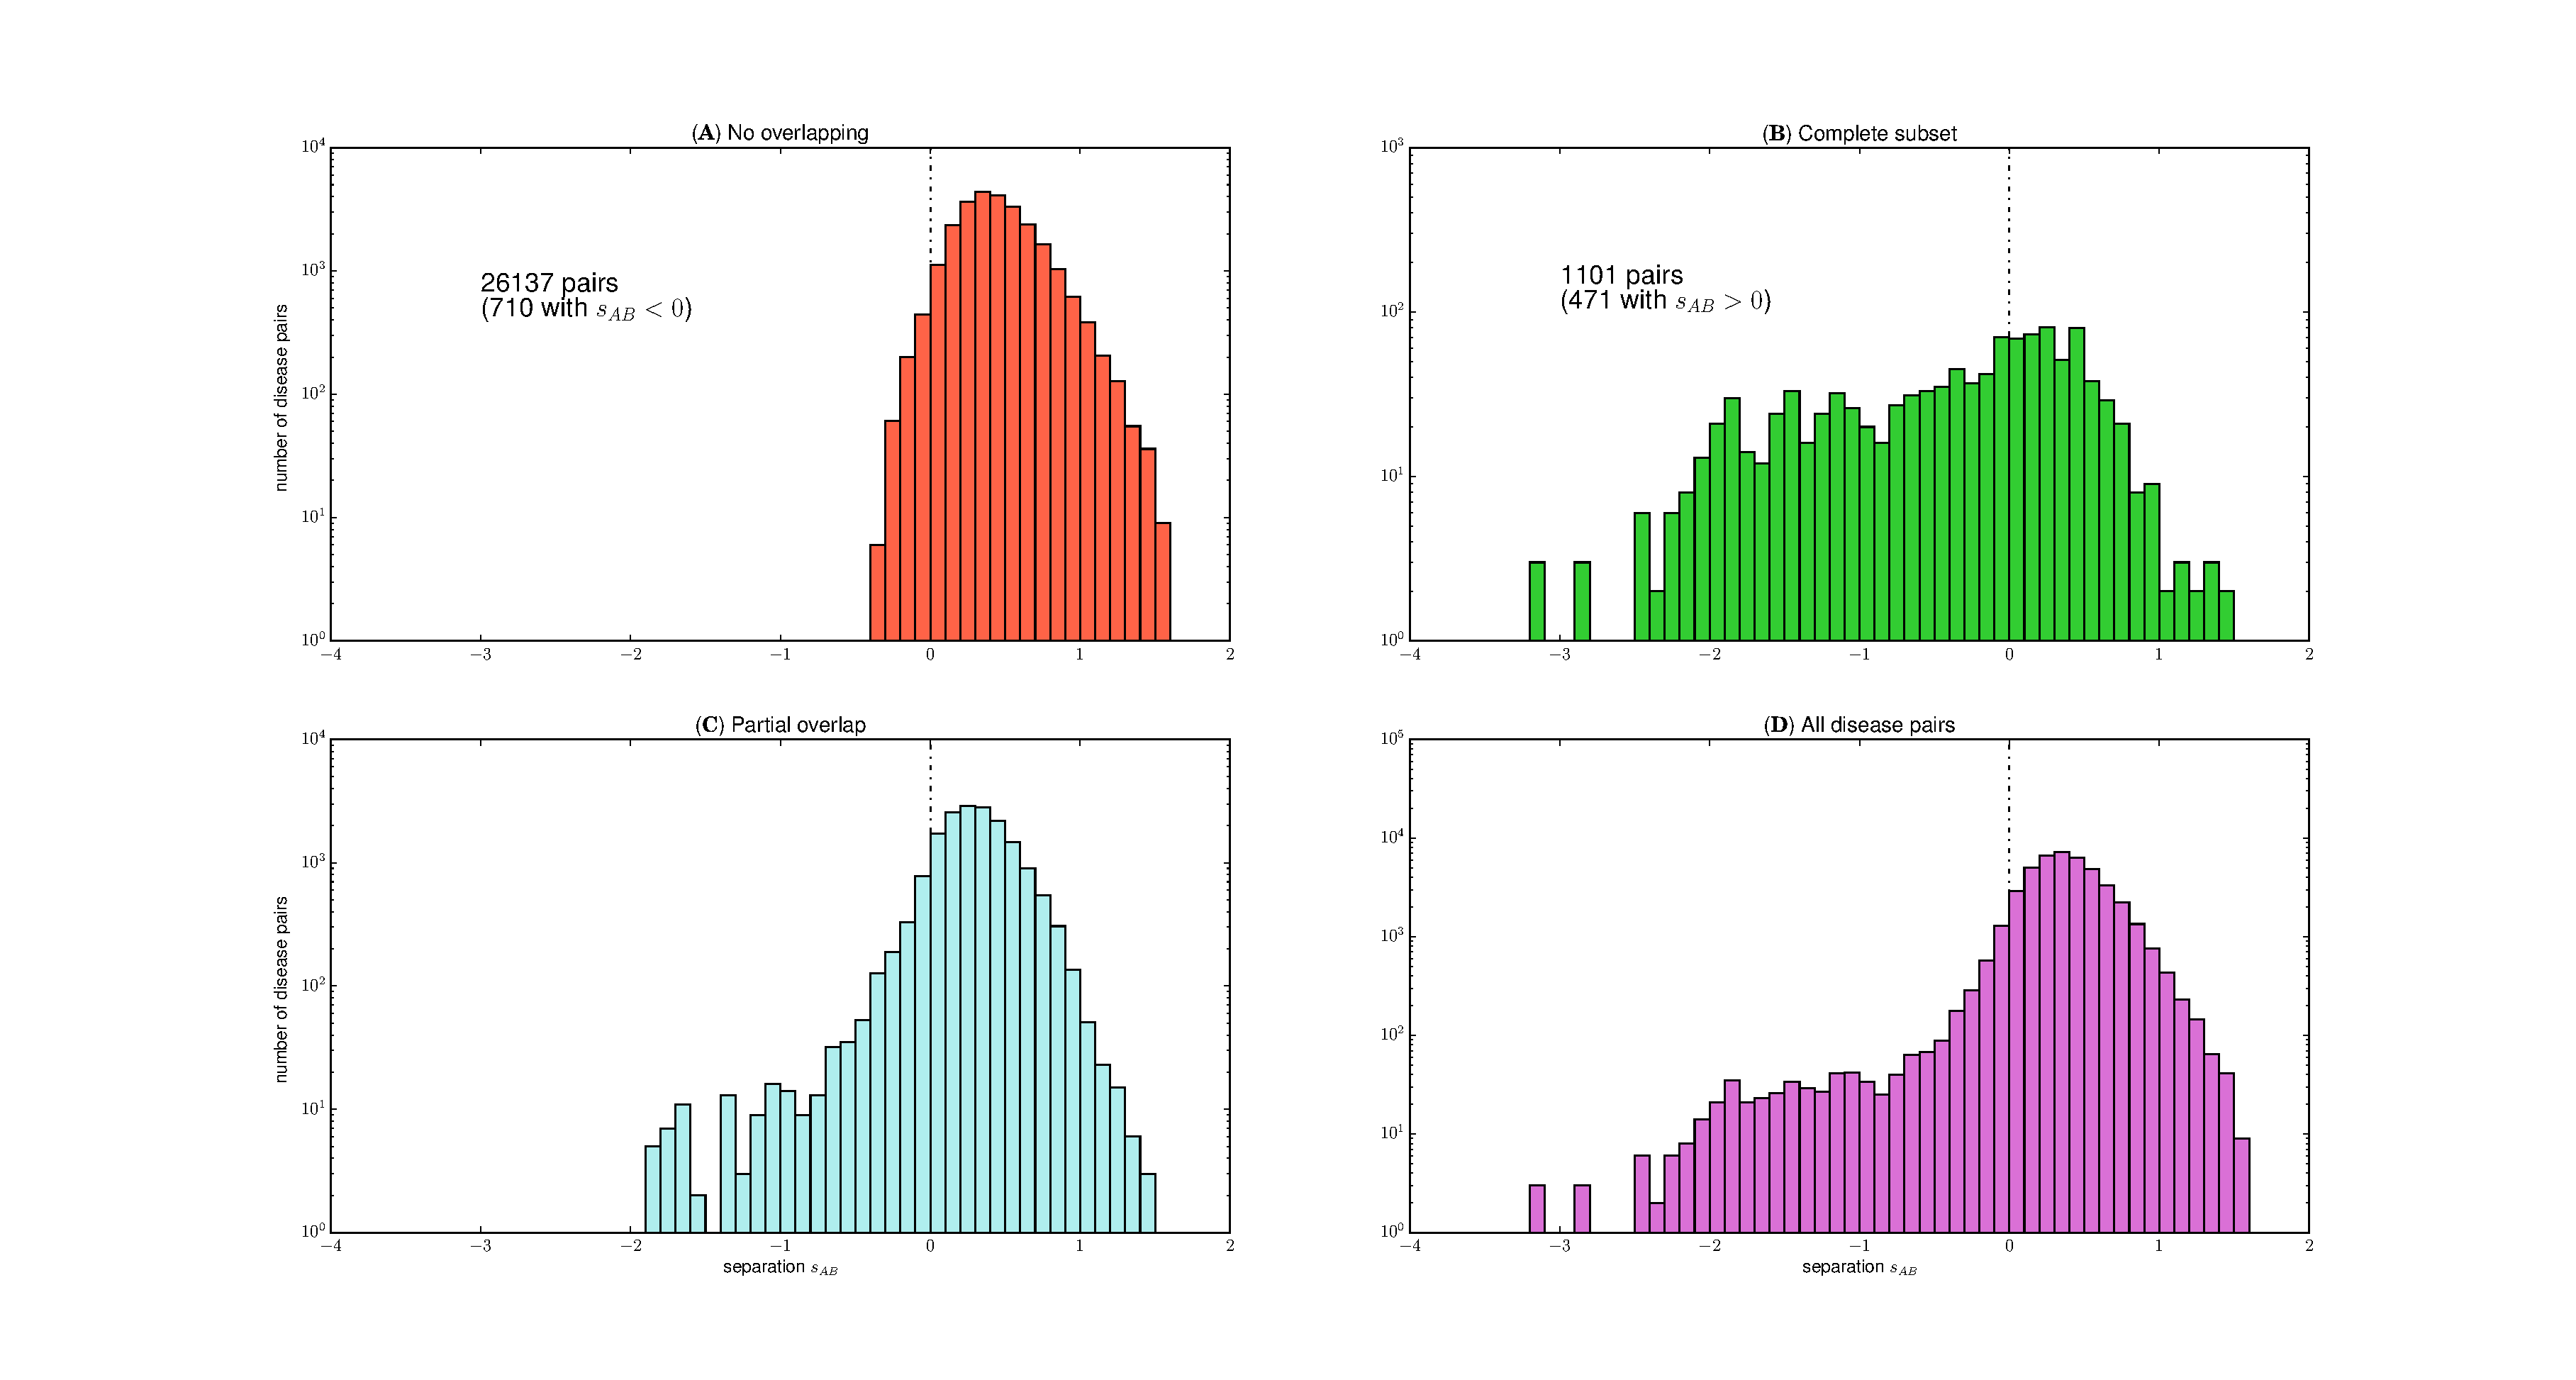
\includegraphics[scale=.35]{images/s_AB_histograms.eps}
			\caption{\label{fig:s_AB histogram}
			{\bf Disease pairs separation.}
			({\bf A}) The $s_{AB}$ distribution of disease pairs with no common gene ($C$-score = $J$-score $= 0$). We
			observe that even though no gene is shared, 710 of the 26,137 pairs (less than $3\%$) have a negative
			separation score (between 0 and 0.5).
			({\bf B}) The $s_{AB}$ distribution of disease pairs with complete overlap ($J$-score $< C$-score $= 1$).
			We observe that despite the inclusion of one disease genes set in the other, 471 of the 1,101 pairs
			(more than $42\%$) have a positive separation score. Yet, separation goes to very low values (below 2).
			({\bf C}) The $s_{AB}$ distribution of disease pairs partially overlapping ($0 < J$-score $ \leq C$-score $< 1$).
			These disease pairs show the same spike of frequency right to $s_{AB} = 0$ as in (A) and the same tail of frequency
			left to $s_{AB} = 0$.
			({\bf D}) The $s_{AB}$ distribution of all the disease pairs.
			}
		\end{figure*}

	\subsection{Robustness}
	We wanted to check if the results of the original paper will still hold with a more recent interactome.
	To reach this aim, we obtained an updated interactome and reproduced the previous analyses with the
	new dataset.

		\subsubsection{Databases update}
		The newer version of the interactome yields a new graph having 17,786 nodes and 370,326 edges, a bit more
		than 1.3 times the initial amount of nodes, and more than 2.6 times the initial amount of edges of the
		original interactome used. From the 4,326 genes added in this newer version, 361 are associated with at
		least one of the 299 diseases, leading to 2,797 disease-associated genes in the interactome versus 2,436
		previously. This reduces the proportion of disease-associated genes of the interactome from $18\%$ in
		the original version to less than $16\%$ in the newer one. Also, the coverage of all the disease-associated
		genes has increased from nearly $77\%$ to more than $88\%$.

		This newer version contains then around $71\%$ of the estimated number of proteins and $57\%$ of the
		estimated interactions of the interactome \citep{estimatingTheSizeOfTheHumanInteractome,ATruerMeasureOfOurIgnorance}.

		Disease genes considered in this update are the same 299 diseases studied in the original paper.
		Further investigation could include also an update of the disease list.

	\subsection{Comparison with original results}
	By defining the density of a graph $\Gamma = (V, E)$ as being $d(\Gamma) \coloneqq \abs E/\binom {\abs V}2$,
	we find that the newer interactome is more than 1.5 times denser than the original one with $0.156\%$ versus $0.234\%$
	for the newer one.

	\subsubsection{Clustering of disease modules}
	We performed the same analysis as previously to study the clustering of the disease modules in the
	interactome with the new version (Figure~\ref{fig:new interactome zscore}). We observed that 12 more
	diseases have a $z$-score below the significance threshold compared to the previous results. We also
	noted a general decrease of the $z$-score.

	\begin{figure}[h!]
		\centering
		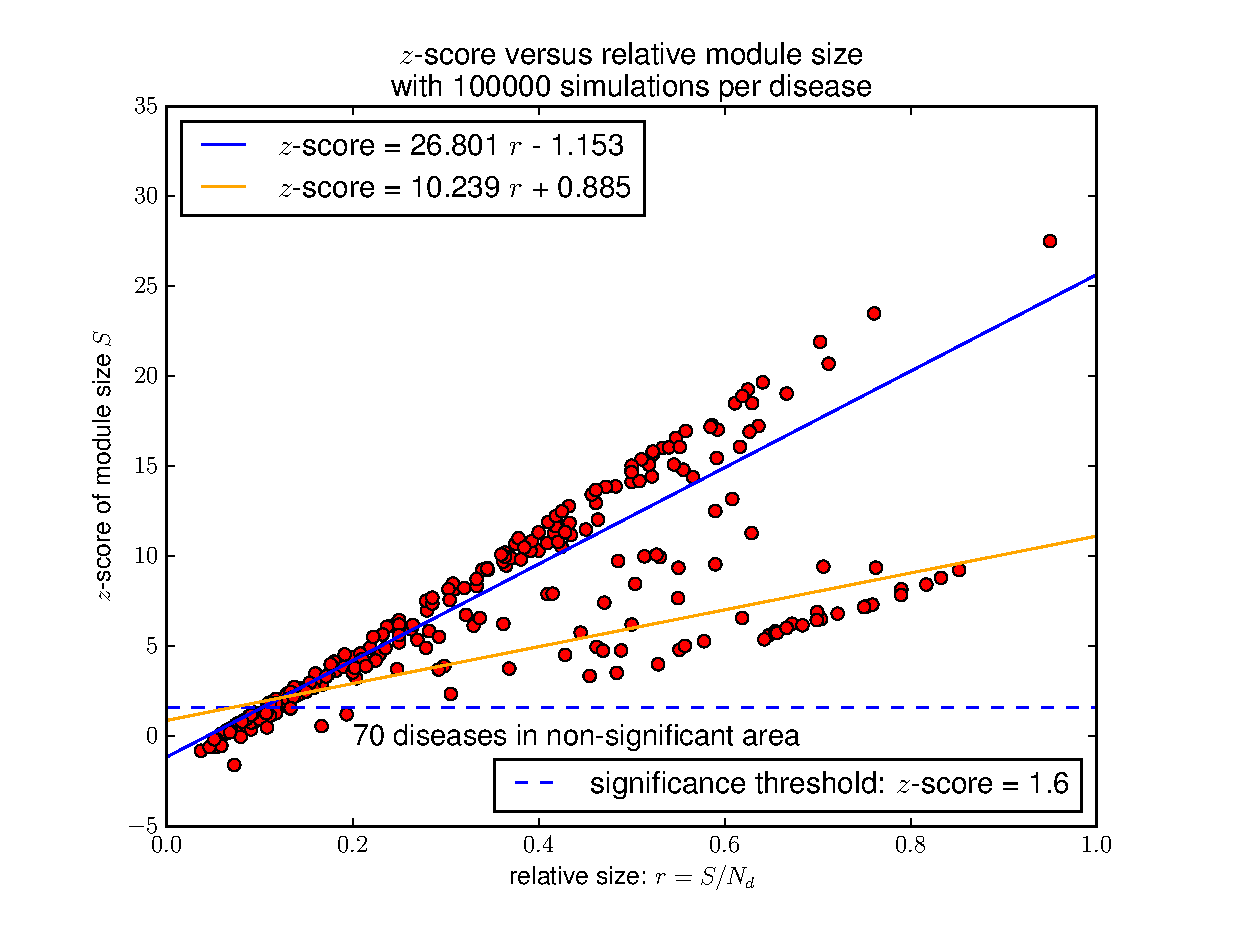
\includegraphics[width=.5\textwidth]{images/new_interactome_S4.b100000.eps}
		\vspace{-.7cm}
		\caption{{\bf z-score of the largest connected component size vs relative module size of the newer interactome.}
		Adaptation of Figure~\ref{fig:zscore} on the new version of the interactome.
		\label{fig:new interactome zscore}}
	\end{figure}

	In order to understand the origin of this decrease in the $z$-score, we compared the relative size
	distribution of the disease modules of the original and the new interactome
	(Figure~\ref{fig:rel sizes comparison}). We noted that the relative size has shifted towards right.

	This can be explained by the increase of the number of genes, leading to a higher coverage of the disease
	modules, and the increase of the number of interaction, leading to a more connected interactome and
	therefore disease modules potentially more connected. Although, the maximum $z$-score has dropped from
	31.6 to 27.5, the mean $z$-score has increased from 6.2 to 6.4 due in part to the increase of the number
	of disease modules with a $z$-score $\in [10, 20]$.

	Another observation was that the average relative size for the given diseases has increased from $22\%$
	to $32\%$ in the new interactome, demonstrating the better coverage brought by the updated version.

	\begin{figure}[!h]
		\centering
		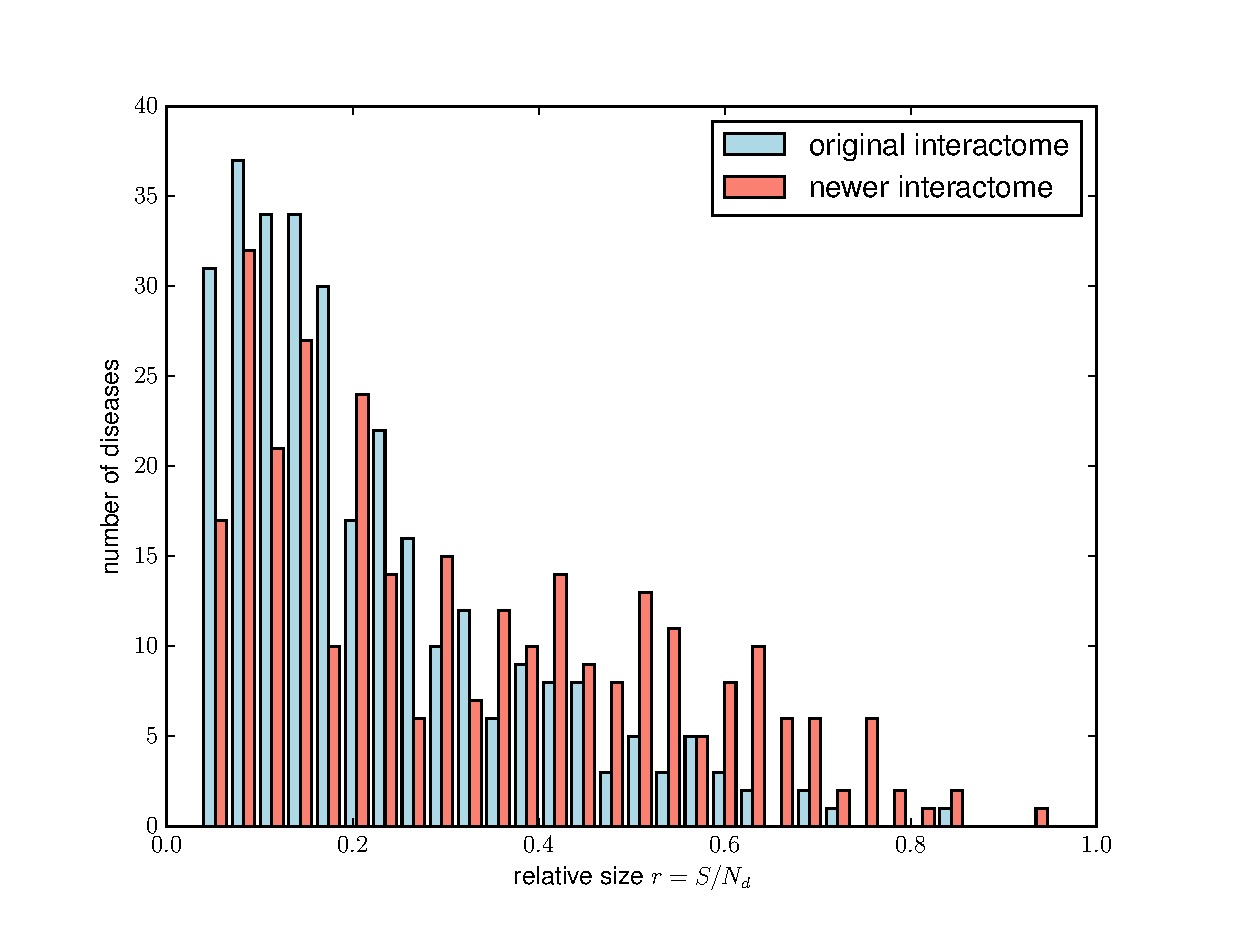
\includegraphics[width=.5\textwidth]{images/rel_sizes_comparison.eps}
		\vspace{-.5cm}
		\caption{{\bf Comparison of relative size distribution between original and newer interactomes.}
		We observe that the number of diseases having a relative size below $\simeq 0.35$ has lowered, whereas the number
		of diseases having a relative size above $\simeq 0.35$ has increased. This is explained by the bigger density of
		the new interactome, leading to larger LCC in the disease subgraphs.
		\label{fig:rel sizes comparison}}
	\end{figure}

	\begin{figure*}[!t]
		\hspace{-1.8cm}
		\vspace{-.5cm}
		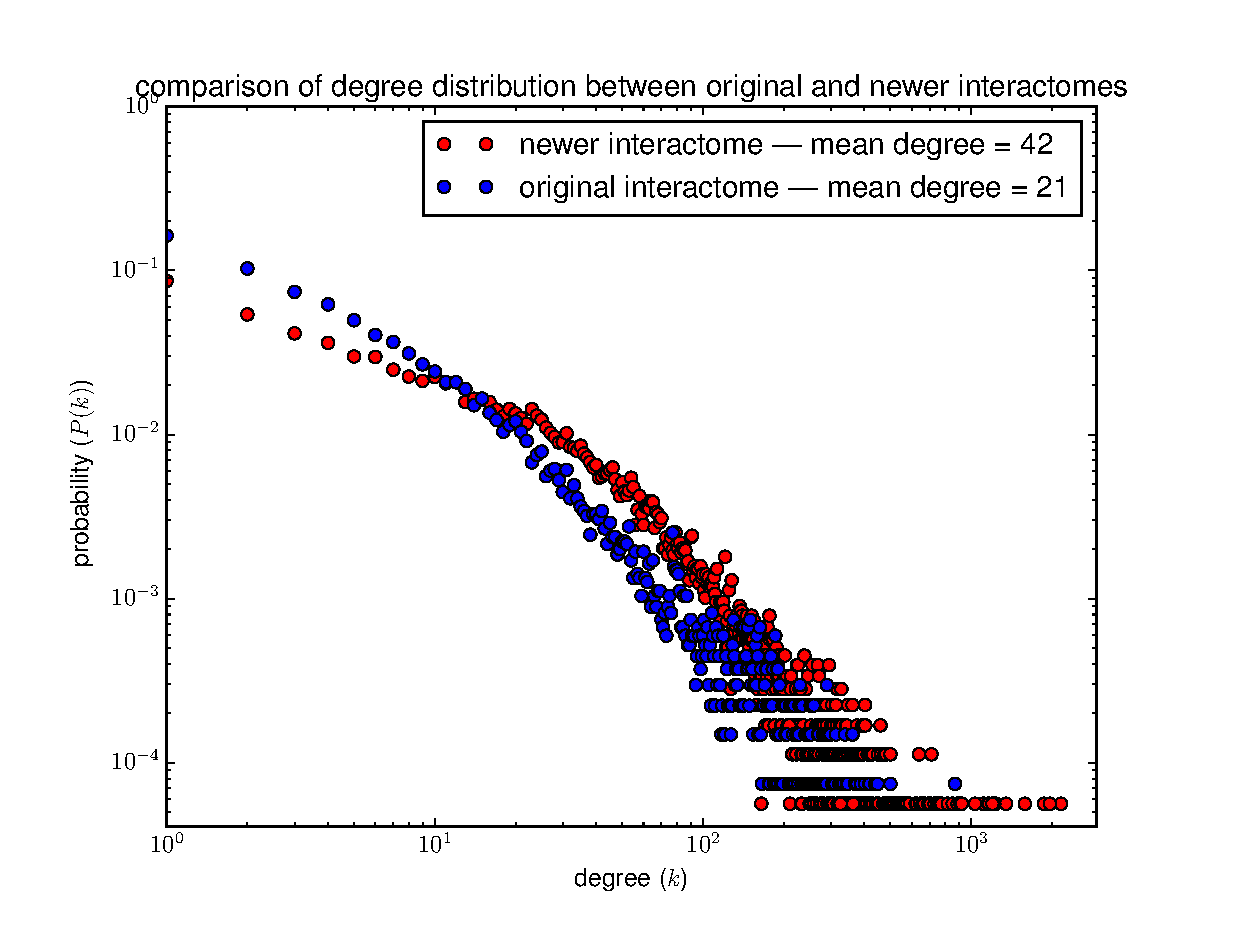
\includegraphics[scale=.45]{images/degree_distributions_comparison.eps}
		\caption{{\bf Degree distribution comparison.} ({\bf A})  Both the original interactome and the new one
		are scale-free, i.e. their degree distribution follows a power law. The power law can be approximated
		with a linear regression according to the relation $\log(P(k)) \sim -\gamma\log(k)$. The new interactome
		has a smaller $\gamma$ coefficient, meaning that a bigger proportion of nodes have a high degree,
		compared to the original one.
		({\bf B}) Cumulative degree distribution of both the original and the newer interactome. We observe
		easily the power law characteristic that even though degree can reach 2,000, almost all the interactome
		nodes have a degree $\leq 100$.
		\label{fig:degree distribution comparison}}
	\end{figure*}

	\begin{figure*}[!b]
		\hspace{-1.8cm}
		\vspace{-1cm}
		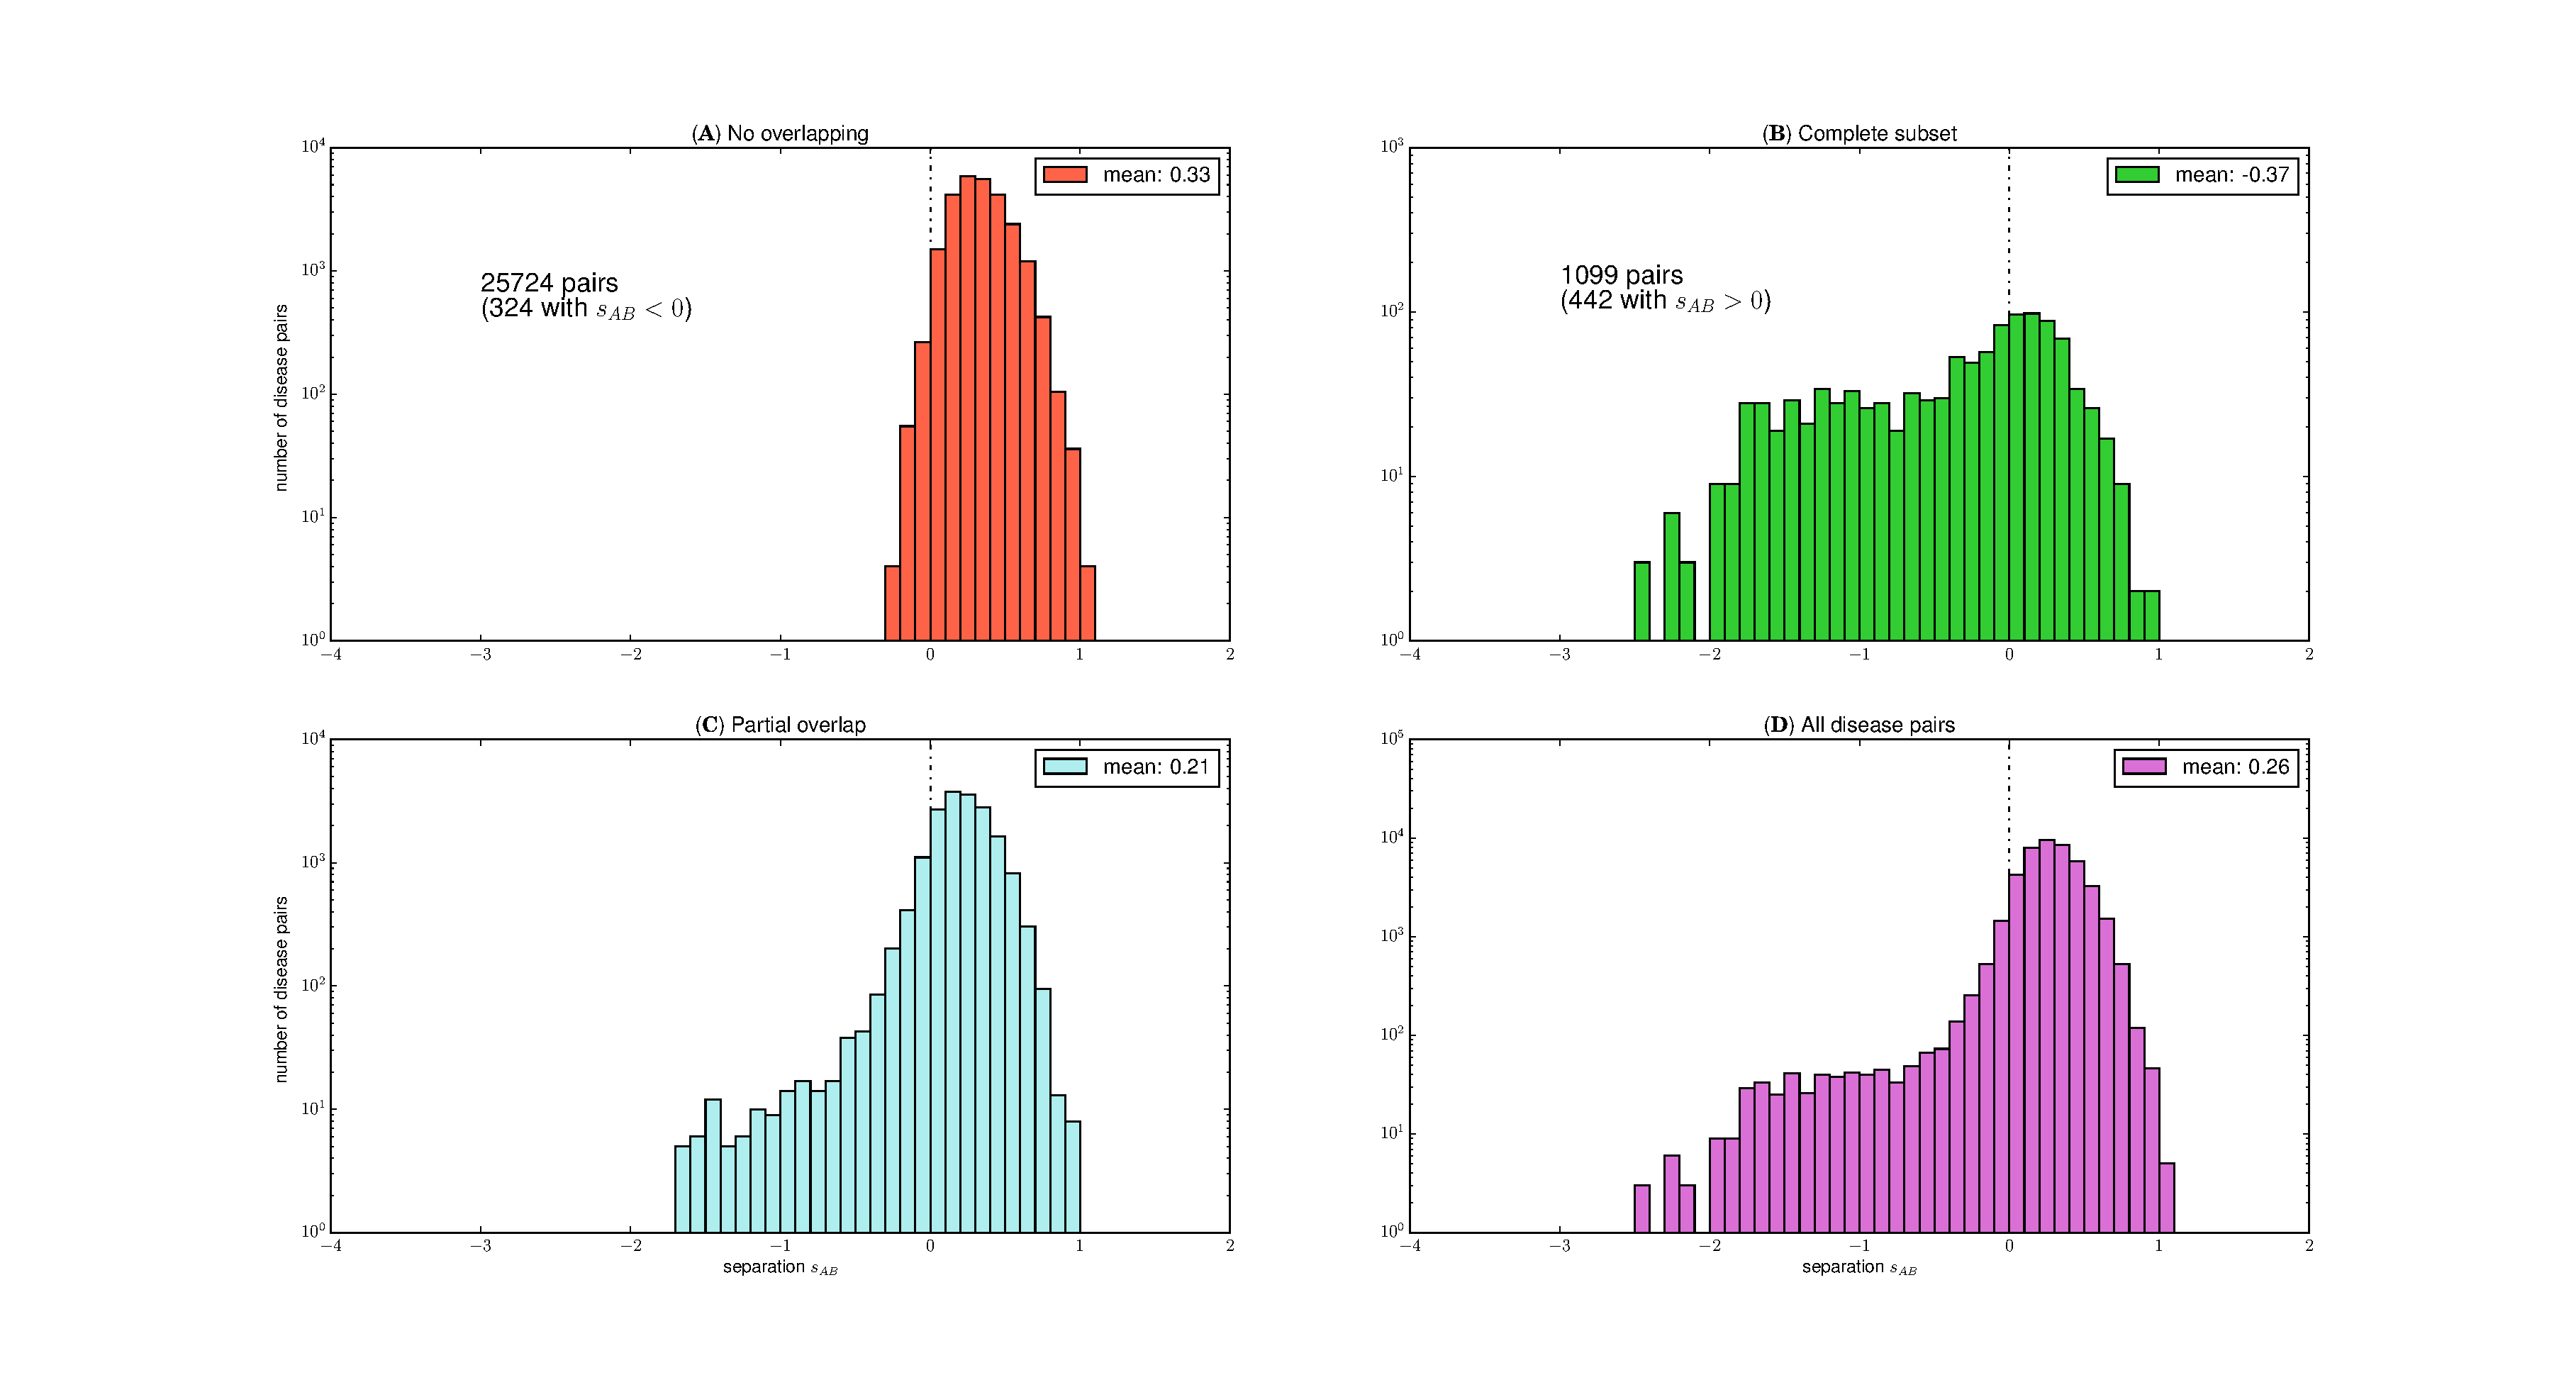
\includegraphics[scale=.35]{images/new_interactome_s_AB_histogram.eps}
		\caption{{\bf Disease pairs separation in the new interactome.} Adaptation of Figure~\ref{fig:s_AB histogram} with the
		updated interactome.
		({\bf A}) We observe that more than half of the disease pairs sharing no genes that had a negative $s_{AB}$ score
		in the original interactome now have a positive score, due to a decrease in $\langle d_A \rangle$ and $\langle d_B \rangle$
		because of the higher density of the newer interactome. ({\bf B}) We also observe that 29 disease pairs related by inclusion
		had a score right shift towards positive values.
		\label{fig:new interactome s_AB}}
	\end{figure*}

	The interpretation of Subsection~\ref{subsec:reproducibility} still stand: diseases having
	a low $z$-score still have a low relative size, and diseases with a higher $z$-score have a higher
	relative size. So either the interactome is still too incomplete for these diseases, or they lie in
	very sparse regions of the interactome. A further investigation of the these diseases and their genes
	is needed to better understand this phenomenon. Due to the graph density increase, the degree
	distribution has changed as well (Figure~\ref{fig:degree distribution comparison}).


	The networks are scale-free, and its degree distribution still follows a power law, which is inherent to
	biological networks. A power law is characterized by a few nodes being highly connected to the other ones,
	whereas most nodes are connected to only a few other ones. We approximated the distribution with a linear
	regression following the relation $\log(P(k)) \sim -\gamma\log(k)$ and determined the $\gamma$ coefficients
	for each distribution. The new interactome has a coefficient of 1.6 while the original one has a coefficient
	of 1.53. The $\gamma$ coefficients are bigger than 1 and smaller than 3, which is considered standard for
	biological networks \citep{UnderstandingTheCellFunctionalOrganization,vidal2011interactome}. This result
	means that while both the original interactome and the new one are highly alike and comparable on their
	degree distribution, the difference is that the new interactome contains more highly connected nodes,
	with a mean twice as big.

	So the decrease of the $z$-score below the threshold of these 12 diseases is also due to the increase of
	the interactome density. The increase in the interactome density implies that a subgraph taken at random
	tends to have a wider LCC at equal size, which is then used for the computation of the $z$-scores.

\subsubsection{Separation distribution}
	When analyzing the separation distribution of the different subgroups of the diseases modules pairs with
	the new interactome (Figure~\ref{fig:new interactome s_AB}), we observed that non-overlapping diseases have
	a higher separation score. With the original interaction, we had 710 disease pairs with a negative separation,
	whereas with the new interactome we observed only 324 pairs with $s_{AB} > 0$ score, meaning that
	$54\%$ of the non-overlapping disease pairs increased their separation score above 0.
	%les modules sont plus souvent séparés physiquement dans l'interactome. Explique pourquoi. Pistes: plus de genes, plus d'interactions ?

	We also observe that $6\%$ of the complete subset disease pairs decreased their separation score below 0,
	however this result is less significant as we observed a large diversity of separation scores for this category.

	When we looked at all the disease pairs together, we observed that separation scores have tightened around 0:
	$s_{AB}$ is in $[-3.2, 1.6]$ in the original interactome, and in the new one, $s_{AB}$ is in $[-2.5, 1.1]$.

	%ajoute peut-être une explication/discussion

\section{Extension of the subgraph largest connected component distribution}
The computation of the z-scores require a null hypothesis. We used here the random hypothesis. The z-scores
are computed as follows: if $S_D$ is the disease module associated with a given disease $D$, then its
$z$-score is given by:
\begin{equation}
	z\text{-score} = \frac {\abs {S_D} - \mu(S^{\text{rand}})}{\sigma(S^{\text{rand}})},
\end{equation}
with $\mu(S^{\text{rand}})$ and $\sigma(S^{\text{rand}})$ being respectively the mean and the standard
deviation of the largest connected component size of a random subgraph of size $\abs D$ in the interactome.

These values are obtained by simulations: taking subgraphs at random of given size in the interactome yields a
distribution $P(S^{\text{rand}})$ with a given mean $\mu(S^{\text{rand}})$ and standard deviation
$\sigma(S^{\text{rand}})$ (Figure~\ref{fig:Srand distribution}).

\begin{figure}[!h]\centering
	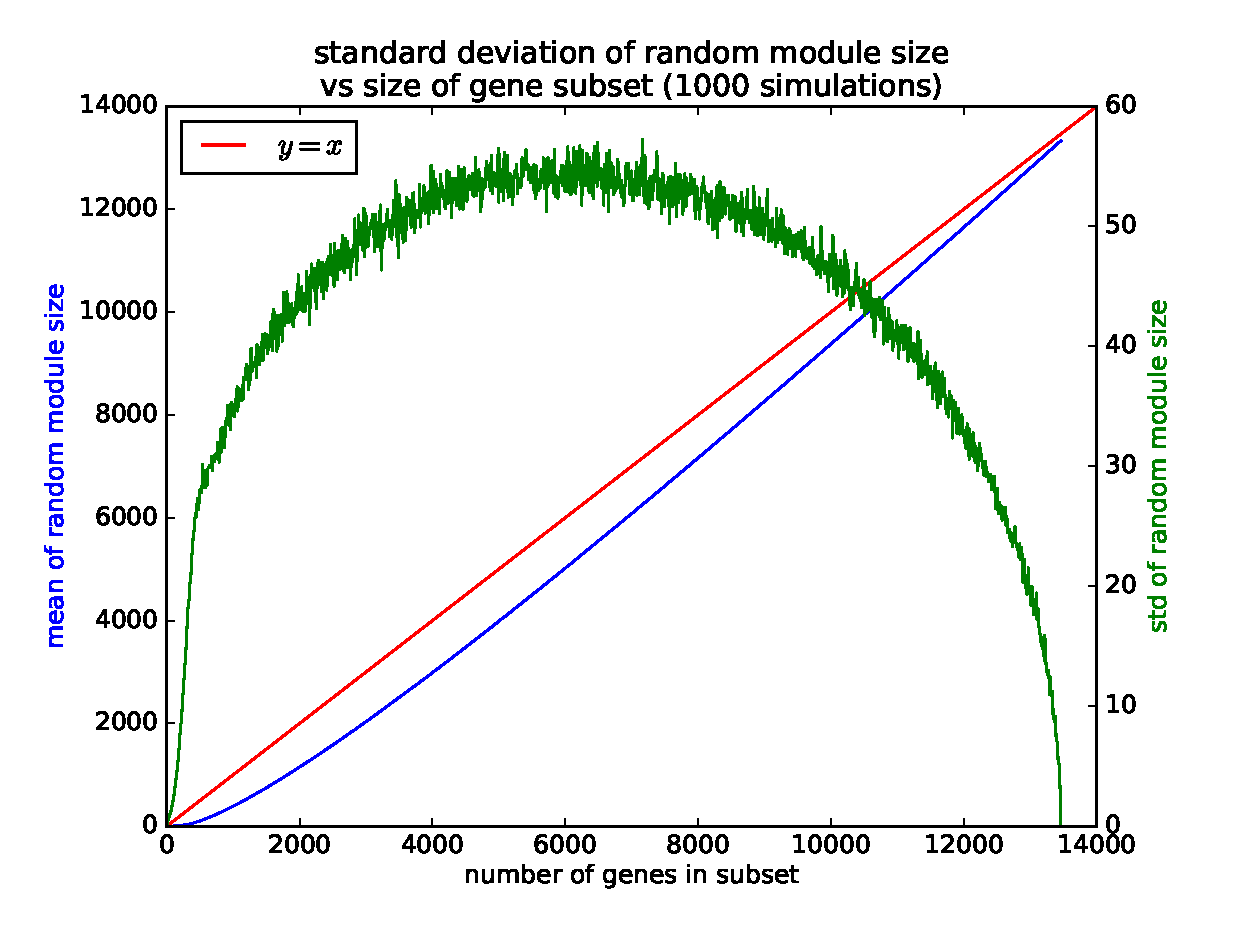
\includegraphics[width=.45\textwidth]{images/Srand_distribution_1000_sims.eps}
	\vspace{-.5cm}
	\caption{{\bf $S^{\text{rand}}$ mean and standard deviation distribution of the original interactome.}
	With $10^3$ simulations per subgraph size, we obtain the distribution of the largest connected component size
	in the interactome. We observe that for subsets of small size $k$, the expected LCC size is significantly smaller than $k$
	whereas for subsets of big size $K$ (giant components), the expected LCC size is much closer to $K$.
	\label{fig:Srand distribution}}
\end{figure}

In order to avoid simulation computation time, we decided to analytically determine the probability density
with a probability mass function. For a graph $\Gamma = (V, E)$ such that $\abs E = m$ and
$\Lambda_k^m(V, \cdot)$, the set of all graphs having $V$ as vertex set, $m$ edges, and a LCC of size $k$,
we define $p_k$, the probability that $\Gamma$ has LCC of size $k$ as:
\begin{equation}
	p_k = \abs {\Lambda_k^m(V, \cdot)}/\binom {\binom {\abs V}2}m,
\end{equation}
which requires $\abs {\Lambda_k^m(V, \cdot)}$ to be computed. However, this set cardinality is defined by a
recurrence relation (see proof in supplementary materials), which makes computations several orders of
magnitude slower, even with dynamic programming and caching, meaning that the time gained by not repeating
the simulation is lost because of the computation time required for the analytical computation.

A Python3 implementation is given in \texttt{source/lcc\_size/}.

\section{Conclusion}

\section{Materials and Methods}
	\subsection{Source code}
	The new version of the interactome and the source code for all plots presented here as well as this
	very paper are available at the following web page: \url{https://github.com/RobinPetit/INFOF-308}.

	\subsection{Database update}
	In order to update the interactome, the tool \textit{inter-tool} \citep{inter-tools} has been used.
	Inter-build (one of the programs from Inter-tools) requires datasets in the PSI-MITAB format, an extension of the
	PSI-MI format \citep{MITABFormat}, and outputs a tsv file.

	The outputted file by Inter-build and the interactome provided with the original paper both use Entrez
	gene IDs, they can therefore easily be merged. In order to merge these, the script \texttt{merger.py}
	has been written. As these two tsv files have a different format (different columns), only the gene IDs
	are outputted by \texttt{merger.py}.

	Latest datasets from BioGRID, IntACT, and the Database of Interacting Proteins (DIP) \citep{salwinski2004DIP}
	(July 25th) and of MINT (July 27th) have been downloaded and merged. The resulting interactome was merged with
	the original one in order to add the interactions to the previous version.

	The others databases cited in Subsection~\ref{subsec:reproducibility} were not included in the newer
	interactome because they were not available for download in a Inter-build-compatible format.

\footnotesize
\bibliographystyle{apalike}
\bibliography{report}{}

\end{document}
